\documentclass[twocolumn,floatfix,aps,prd,nofootinbib]{revtex4-2}

\usepackage[utf8]{inputenc}
\usepackage[T1]{fontenc}
\usepackage{graphicx}
\usepackage{amssymb}
\usepackage{amsmath}
\usepackage{xcolor}
\usepackage{hyperref}
\usepackage{textcase}
\usepackage{placeins}
\usepackage[protrusion=true,expansion=false]{microtype}

\hypersetup{
    colorlinks=true,
    linkcolor=blue,
    filecolor=magenta,
    urlcolor=blue,
    citecolor=blue,
}
\urlstyle{same}
\emergencystretch=2em

\begin{document}

\title{\texorpdfstring{\MakeTextUppercase{Neural Spacetime Search with \texttt{GRTeclyn}: A Practical Baseline for Dynamical Metric Discovery}}{Neural Spacetime Search with GRTeclyn: A Practical Baseline for Dynamical Metric Discovery}}

\author{\MakeTextUppercase{Nikita M. Shirokov}}
\email{shirokov.nm@phystech.edu}
\affiliation{\textit{Independent Researcher, Moscow, Russia}}
\date{\today}

\begin{abstract}
We outline a practical baseline for turning \texttt{GRTeclyn} into a closed-loop GPU search engine for exotic spacetime metrics. A Python scheduler proposes compact initial-data parameters, a C++/AMReX executable evolves each candidate, and scoring diagnostics promote only geometries that survive, show operational faster-than-light (FTL) benefit, and avoid coordinate artifacts. Matter is handled either by algebraic reconstruction from the Einstein constraints at $t=0$ or, in the long-term path, by an elliptic positive-energy initial-data solve.
\end{abstract}

\maketitle

\section{Introduction}

Most proposed interstellar metrics are hand-designed static ans\"atze.  That approach is analytically clean but strongly biased toward highly symmetric geometries.

Here metric discovery is treated as black-box optimization over dynamical 3D initial data.  The framework couples a Python optimizer to the GPU AMR evolution engine in \texttt{GRTeclyn}, with explicit checks for matter consistency, stability, and fake-FTL gauge effects.

This fits a broader shift toward automated theory exploration~\cite{alexander2026albert,halverson2019branes,qiu2026collideragent,han2025physagent}.  For warp geometries, \textsc{Warp Factory} and \textsc{warpax} emphasize observer-robust energy-condition evaluation~\cite{helmerich2024warpfactory,le2026warpax}; we extend that philosophy from analysis of prescribed metrics to search over evolved initial data, while keeping numerical convergence and constraint satisfaction central~\cite{lousto2006fourth,li2023pinn}.

Throughout this draft, ``FTL'' means effective faster-than-light propagation through a curved spacetime geometry compared with flat-spacetime light travel. It does not imply local superluminal motion relative to the local light cone.

\section{Goal}

The goal is an automated numerical-relativity laboratory for FTL transport, FTL communication, portal-like shortcuts, and wormhole throats.  A successful candidate must survive evolution, show an operational shortcut relative to a flat control, keep tidal forces bounded, and minimize violations of the standard energy conditions.

\subsection{Optimization as the Engine of Discovery}

Blind random 3D initial data almost always violates constraints, collapses, or relaxes to flat space.  Optimization supplies the steering: maximize FTL benefit while penalizing constraint error, negative energy, tidal force, and instability.

\section{Initial Data and Matter Derivation}

The initial spatial metric $\gamma_{ij}$ and extrinsic curvature $K_{ij}$ must satisfy the Einstein constraints, which determine the compatible energy density $\rho$ and momentum density $j_i$.  We use two matter-sector paths:

\subsection{Path A: Algebraic Matter Reconstruction}

The optimizer proposes geometry; the constraints give its required matter cost,
\begin{equation}
    \rho = \frac{R + K^2 - K_{ij}K^{ij}}{16\pi},\qquad
    j_i = \frac{1}{8\pi} D_j\!\left(K^j_i - \delta^j_i K\right),
\end{equation}
with $R$ the 3D Ricci scalar and $D_j$ the covariant derivative.  Regions with $\rho<0$ are recorded as exotic-matter cost and fed back into the objective.

\subsection{Path B: Elliptic Constraint Solving}

The longer-term positive-energy path fixes a matter model with $\rho\ge0$ and uses an elliptic solver (e.g.\ \texttt{GRTresna}) to deform each proposed geometry until the constraints are satisfied before evolution.

\section{Candidate Parameterization}

The optimizer emits a compact vector $\theta$; a decoder maps it to smooth AMReX initial fields.

\subsection{Level 1: Radial Recipes}

We define the initial fields at $t=0$ using spherically symmetric radial profiles:
\begin{equation}
    q(r) = q_\infty + \sum_n a_n B_n(r),
\end{equation}
where $q$ denotes $\chi$, $\alpha$, $\beta^i$, or $K$, and $B_n$ are smooth radial basis functions.

\subsection{Level 2: Angular Recipes (implemented)}

Angular modes add non-spherical structure:
\begin{equation}
    q(r,\theta,\varphi) = q_\infty + \sum_{n\ell m} a_{n\ell m}B_n(r)Y_{\ell m}(\theta,\varphi).
\end{equation}
This is implemented for gauge fields ($\alpha,\beta^i$), where angular modes carry no constraint cost; geometric angular modes require the future 3D constraint solver.

\subsection{Levels 3--4: Neural and Meta-Optimization (future)}
\label{sec:parameterization_levels}

Future Level~3 replaces basis functions with an implicit neural decoder, optionally trained with Hamiltonian and momentum residuals as PINN losses~\cite{li2023pinn}.

\paragraph{A symbolic ``spacetime grammar'' (neuro-symbolic constraint filtering).}
A rule-based spacetime grammar can enforce asymptotic flatness, positivity, $K=\mathrm{const}$, $\Pi=0$, and chosen topology before evaluation, reducing wasted GPU jobs in the spirit of grammar-constrained theory generation~\cite{alexander2026albert}.

\paragraph{Level 4: a concrete LLM meta-agent.}
Level~4 is an LLM meta-agent that classifies failed runs, retunes exposed gauge/grid parameters, and proposes new modes while leaving the physics verdict to read-only diagnostics~\cite{qiu2026collideragent}.

\section{GPU Cluster Architecture and Program Boundary}

The pipeline keeps Python orchestration separate from precompiled GPU evolution: Python proposes and scores candidates; the C++ executable only loads parameters, initializes fields, evolves, and writes diagnostics.

\subsection{The Execution Boundary}

The Python controller writes \texttt{params.txt} and dispatches Slurm tasks; GPU nodes run the same \texttt{GRTeclyn} binary for every candidate, avoiding recompilation inside the search loop.

\subsection{Tiered GPU Execution}

Tier~1 uses short low-resolution single-GPU runs with early stopping; Tier~2 promotes survivors to multi-GPU resolution ladders for stability and convergence.

\section{The Closed-Loop: How Simulation Results Drive the Search}
\label{sec:closed_loop}

Each optimizer evaluation follows:

\begin{enumerate}
    \item propose basis coefficients $\theta$;
    \item derive constrained fields, write \texttt{params.txt}, and reject bad pre-flight residuals;
    \item evolve on GPU and write constraint, collapse, matter, and plotfile diagnostics;
    \item parse diagnostics into $S(\theta)$ and update CMA-ES after each generation.
\end{enumerate}

The optimizer sees only the scalar black-box objective $f(\theta)=-S(\theta)$, making the score design the central physics interface.

\section{Scoring: Overcoming the Flat-Space Attractor}
\label{sec:scoring}

The score must reward FTL-relevant structure without letting trivial Minkowski win by being perfectly stable and constraint-clean.  The upgraded objective therefore adds continuous FTL scaffolding ($F_{\rm asymmetry}$, $F_{\rm log}$), co-moving stability, growth penalties, and a non-triviality gate.

\subsection{Implemented score components}

Each component $s_k$ is mapped through
\begin{equation}
    r(v;\,\sigma) = \frac{1}{1 + v/\sigma},
    \label{eq:bounded_reward}
\end{equation}
and combined as
\begin{equation}
    S(\theta) = \sum_{k} w_k\,s_k(\theta).
\end{equation}

\subsection{Continuous FTL scaffolding metrics}
\label{sec:ftl_scaffolding}

Two continuous proxies give CMA-ES a gradient before a fully superluminal candidate appears.

\subsubsection{Nat\'{a}rio--Alcubierre expansion asymmetry}

For a warp-like contraction-ahead/expansion-behind pattern, use
\begin{equation}
    F_{\rm asymmetry} = \max\!\left(0,\, \frac{\int_{x > 0} -\theta(\mathbf{x})\,d^3x + \int_{x < 0} \theta(\mathbf{x})\,d^3x}{\int |\theta(\mathbf{x})|\,d^3x + \epsilon_{\theta}} \right).
\end{equation}
The implemented 1D evaluator reduces these integrals to trapezoidal sums along the travel axis.

\subsubsection{Logarithmic FTL amplification}

Weak shortcuts are log-amplified:
\begin{equation}
    F_{\rm log} = \frac{\ln(1 + \eta F_{\rm FTL})}{\ln(1 + \eta)},
    \label{eq:f_log}
\end{equation}
with $\eta\approx100$, so even a few-percent shortcut becomes optimizer-visible.

\subsection{Co-moving stability scoring}
\label{sec:comoving_scoring}

Eulerian stability penalizes moving bubbles.  We therefore estimate stability in a co-moving frame.

The average axial shift is
\begin{equation}
    \langle \beta^x \rangle = \frac{1}{V_{\rm bubble}} \int_{\rm bubble} \beta^x(\mathbf{x})\,d^3x.
\end{equation}
and the co-moving budget is
\begin{align}
    \Delta_{\rm comoving}
    &= \frac{\max_t \left| \partial \chi / \partial t \right|}
            {\max(|\langle \beta^x \rangle|,\,10^{-3})}, \notag\\
    s_{\rm comoving}
    &= \frac{1}{1 + \Delta_{\rm comoving}}.
    \label{eq:s_comoving}
\end{align}
For stationary throats or portals with negligible shift, \texttt{score.py} falls back to Eulerian stability.

\begin{table*}[t]
\caption{Compact score-weight summary.  Components are inactive when their diagnostics are unavailable.}
\label{tab:score_weights}
\small
\begin{ruledtabular}
\begin{tabular}{lp{0.72\textwidth}}
Group & Weights \\
\hline
FTL value & $5F_{\rm log}+2F_{\rm asymmetry}+s_{\rm nonflat}+3F_{\rm op}$ \\
Health & $1.5s_{\rm survival}+2s_{\rm constraints}+s_{\rm lapse}+2.5s_{\rm comoving}+0.5s_{\rm stability}$ \\
Risk penalties & $1.5s_{\rm horizon}+2s_{\rm EC}+2s_{\rm growth}+1.5s_{\rm anec}+s_{\rm tidal}$ \\
Evolved geometry & $0.5F_{\rm curv}+1.5s_{\rm exotic}^{\rm eff}$ \\
\end{tabular}
\end{ruledtabular}
\end{table*}
Unavailable diagnostics contribute zero, so legacy episodes re-score consistently.

\subsubsection{The non-triviality gate: defeating the flat-space attractor}
\label{sec:nontriviality_gate}

Health rewards are multiplied by a non-triviality gate so flat space cannot win solely by being clean:
\begin{equation}
    \begin{aligned}
    g_{\rm nt} = \min\!\Bigl(1,\ \max\bigl(&s_{\rm nonflat},\,F_{\rm asymmetry},\,s_{\rm nontrivial},\\
    &F_{\rm curv},\,F_{\rm op},\,F_{\rm log},\,s_{\rm exotic}^{\rm eff}\bigr)\Bigr)\in[0,1],
    \end{aligned}
\end{equation}
The health rewards $\mathcal{H}$ are gated, while FTL/exoticity terms remain ungated:
\begin{equation}
    S(\theta) = g_{\rm nt}(\theta)\!\!\sum_{k\in\mathcal{H}}\!\! w_k s_k(\theta)\ +\!\!\sum_{k\notin\mathcal{H}}\!\! w_k s_k(\theta).
    \label{eq:gated_score}
\end{equation}
With this gate, flat Minkowski drops to $S=0$ while structured reference geometries keep their original scores.

\subsection{FTL shortcut metrics (implemented)}
\label{sec:ftl_scoring}

\texttt{ftl\_metrics.py} reconstructs $t=0$ profiles and evaluates three shortcut indicators on the $x$-axis.

\subsubsection{Warp null-ray shortcut}

For conformally flat slices, an axial null ray has
\begin{equation}
    \frac{dx}{dt} = \alpha(x)\sqrt{\chi(x)} - \beta^x(x).
\end{equation}
with travel time
\begin{equation}
    T_{\rm curved} = \int_{-L}^{L}\frac{dx}{\alpha\sqrt{\chi}-\beta^x}, \qquad
    T_{\rm flat} = 2L,
\end{equation}
and reward
\begin{equation}
    F_{\rm null} = \max\!\left(0,\,\frac{T_{\rm flat}-T_{\rm curved}}{T_{\rm flat}}\right).
\end{equation}
Paths below a coordinate-speed floor are rejected.

\subsubsection{Portal proper-distance shortcut}

The portal-like compression reward is
\begin{align}
    D_{\rm proper}
    &= \int_{-L}^{L}\chi^{-1/2}(r)\,dr, \notag\\
    F_{\rm portal}
    &= \max\!\left(0,\,\frac{2L-D_{\rm proper}}{2L}\right),
\end{align}

\subsubsection{Wormhole throat pinch}

The throat reward compares an interior areal-radius minimum to the asymptotic radius:
\begin{equation}
    F_{\rm throat} = \max\!\left(0,\,1-\frac{R_{\rm min}}{R_{\rm asymp}}\right).
\end{equation}

\subsubsection{Anti-flatness and combined objective}

The anti-flat gate is
\begin{equation}
    s_{\rm nonflat} = \min\!\left(1,\,\frac{\max|\chi-1|+\max|\beta^x|}{\tau}\right),
\end{equation}
with scale $\tau\sim0.08$, giving
\begin{equation}
    F_{\rm FTL} = \max(F_{\rm null},F_{\rm portal},F_{\rm throat})\cdot s_{\rm nonflat}.
\end{equation}
The optimizer uses $F_{\rm log}$ rather than raw $F_{\rm FTL}$.

\subsubsection{Validation: FTL scoring across reference seeds}

Table~\ref{tab:ftl_validation} checks the reference seeds at $L=8$.

\begin{table}[tbp]
\caption{FTL metric scores for reference spacetime seeds ($L=8$).  Raw $F_{\rm FTL}=\max(F_{\rm null},F_{\rm portal},F_{\rm throat})\cdot s_{\rm nonflat}$; $F_{\rm log}$ from Eq.~\ref{eq:f_log} with $\eta=100$.}
\label{tab:ftl_validation}
\small
\begin{ruledtabular}
\begin{tabular}{lcccccc}
Seed & $F_{\rm null}$ & $F_{\rm FTL}$ & $F_{\rm log}$ & $F_{\rm asym}$ & $s_{\rm nonflat}$ \\
\hline
Flat Minkowski & 0 & 0 & 0 & 0 & 0 \\
Alcubierre $v=0.3$ & 0.063 & 0.063 & 0.432 & 0.083 & 1.0 \\
Alcubierre $v=0.5$ & 0.094 & 0.094 & 0.508 & 0.083 & 1.0 \\
Alcubierre $v=0.8$ & 0.131 & 0.131 & 0.573 & 0.083 & 1.0 \\
Ellis--Bronnikov (16 bases) & 0 & 0.945 & 0.988 & 0.998 & 1.0 \\
Schwarzschild & 0 & 0.878 & 0.972 & 0.999 & 1.0 \\
\end{tabular}
\end{ruledtabular}
\end{table}

The log term makes subluminal Alcubierre signals visible, while throat-like seeds score through proper-distance and asymmetry channels even when $F_{\rm null}=0$.

\subsubsection{Why FTL scoring resolves the flat-space attractor}
\label{sec:ftl_attractor}

The three shortcut channels are independent: shift-driven warp, $\chi>1$ compression, and areal-radius throat pinching.  The nine-dimensional default search vector in Table~\ref{tab:search_space} spans these mechanisms while remaining tractable.

\begin{table}[tbp]
\caption{CMA-ES search dimensions with bounds.  All coefficients are dimensionless amplitudes for the Gaussian basis expansion.}
\label{tab:search_space}
\small
\begin{ruledtabular}
\begin{tabular}{lccc}
Parameter & Lower & Upper & Initial \\
\hline
\texttt{recipe\_chi\_coeff\_0} & $-0.5$ & $0.1$ & $-0.1$ \\
\texttt{recipe\_chi\_coeff\_1} & $-0.3$ & $0.3$ & $0$ \\
\texttt{recipe\_chi\_coeff\_2} & $-0.2$ & $0.2$ & $0$ \\
\texttt{recipe\_chi\_coeff\_3} & $-0.2$ & $0.2$ & $0$ \\
\texttt{recipe\_basis\_width} & $0.3$ & $3.0$ & $1.0$ \\
\texttt{recipe\_alpha\_coeff\_0} & $-0.3$ & $0.3$ & $0$ \\
\texttt{recipe\_alpha\_coeff\_1} & $-0.3$ & $0.3$ & $0$ \\
\texttt{recipe\_beta\_coeff\_0} & $-0.5$ & $0.5$ & $0$ \\
\texttt{recipe\_beta\_coeff\_1} & $-0.5$ & $0.5$ & $0$ \\
\end{tabular}
\end{ruledtabular}
\end{table}

\subsubsection{GPU validation with upgraded FTL scoring}
\label{sec:gpu_ftl_validation}

Completed GPU smoke episodes were re-scored with the upgraded objective.

\paragraph{Reference seeds: flat-space attractor resolved.}
Table~\ref{tab:gpu_ftl_upgraded} shows the key result: Alcubierre $v=0.5$ outranks flat Minkowski because $F_{\rm log}$ and $s_{\rm comoving}$ offset the Eulerian stability penalty.

\begin{table*}[t]
\caption{GPU smoke results with upgraded FTL scoring ($t=2$, $N_{\rm full}=64$, $L=8$).  Scores recomputed from archived episodes with \texttt{score.py} weights from Table~\ref{tab:score_weights}.}
\label{tab:gpu_ftl_upgraded}
\small
\begin{ruledtabular}
\begin{tabular}{lccccc}
Candidate & $F_{\rm log}$ & $F_{\rm asym}$ & $s_{\rm comoving}$ & $s_{\rm stability}$ & $S$ \\
\hline
Alcubierre $v=0.5$ & 0.508 & 0.083 & 0.998 & 0.02 & \textbf{10.08} \\
Flat Minkowski & 0 & 0 & 1.000 & 1.00 & 10.00 \\
Ellis--Bronnikov ($N{=}16$) & 0.988 & 0.998 & 0.074 & 0.07 & \textbf{10.84} \\
\texttt{random\_angular\_004} & 0 & 0.989 & 0.019 & 0.50 & 6.43 \\
\texttt{random\_000} & 0 & 0.391 & 0.015 & 0.46 & 3.91 \\
\texttt{random\_003} & 0.174 & 0.476 & 0.023 & 0.02 & 3.76 \\
\end{tabular}
\end{ruledtabular}
\end{table*}

The same scoring keeps random $\chi$-only angular candidates below validated warp/throat seeds.

\paragraph{Non-spherical angular candidates.}
Table~\ref{tab:gpu_ftl_nonspherical} shows that non-spherical $\chi$ deformations produce strong asymmetry but no axial null shortcut.

\begin{table*}[t]
\caption{Non-spherical GPU batch with upgraded FTL scoring ($t=2$, $N_{\rm full}=64$, stamp \texttt{20260528\_151713}).}
\label{tab:gpu_ftl_nonspherical}
\small
\begin{ruledtabular}
\begin{tabular}{lccccc}
Candidate & $F_{\rm log}$ & $F_{\rm asym}$ & $s_{\rm comoving}$ & $s_{\rm stability}$ & $S$ \\
\hline
\texttt{random\_angular\_004} & 0 & 0.989 & 0.019 & 0.50 & 6.43 \\
\texttt{random\_angular\_007} & 0 & 0.989 & 0.020 & 0.51 & 6.13 \\
\texttt{quadrupole\_bubble\_001} & 0 & 0.989 & 0.019 & 0.50 & 6.14 \\
\texttt{random\_angular\_005} & 0 & 0.989 & 0.019 & 0.49 & 6.14 \\
\texttt{random\_angular\_006} & 0 & 0.989 & 0.019 & 0.49 & 6.15 \\
\texttt{dipole\_lopsided\_000} & 0 & 0.989 & 0.015 & 0.44 & 6.16 \\
\texttt{mixed\_modes\_002} & 0 & 0.989 & 0.015 & 0.44 & 6.12 \\
\end{tabular}
\end{ruledtabular}
\end{table*}

These campaigns establish the baseline: shift-enabled warps can exceed flat space, while angular $\chi$ deformations plateau on asymmetry alone.

\subsection{Dynamical stability scoring (implemented)}
\label{sec:stability_scoring}

Short runs can survive while already focusing toward collapse.  We therefore score geometry growth explicitly instead of relying on survival time alone.

\subsubsection{Data sources}

The metric uses \texttt{collapse\_diagnostics.dat} and \texttt{areal\_radius.dat}: $\alpha_{\min}$, $\chi_{\min}$, $|K|_{\max}$, $r_H$, and $R_{\rm areal}$ over the full run.

\subsubsection{Fractional violation terms}

For each sampled diagnostic,
\begin{align}
    \Delta q_{\rm grow}
    &\equiv \frac{\max_t q(t) - q(0)}
            {\max\!\bigl(|q(0)|,\,q_{\rm floor}\bigr)}, \notag\\
    \Delta q_{\rm drop}
    &\equiv \frac{q(0) - \min_t q(t)}
            {\max\!\bigl(|q(0)|,\,q_{\rm floor}\bigr)},
\end{align}
with terms clipped to $\ge0$.  The implemented indicators are:
\begin{align}
    \Delta_K &\equiv \Delta\bigl(|K|_{\max}\bigr)_{\rm grow}
    \quad\text{with } q_{\rm floor} = 10^{-1}, \label{eq:delta_k}\\
    \Delta_\alpha &\equiv \Delta\bigl(\alpha_{\min}\bigr)_{\rm drop}
    \quad\text{with } q_{\rm floor} = 10^{-6}, \label{eq:delta_alpha}\\
    \Delta_\chi &\equiv \Delta\bigl(\chi_{\min}\bigr)_{\rm drop}
    \quad\text{with } q_{\rm floor} = 10^{-8}, \label{eq:delta_chi}\\
    \Delta_{r_H} &\equiv \Delta\bigl(r_H\bigr)_{\rm grow}
    \quad\text{with } q_{\rm floor} = 1, \label{eq:delta_rh}\\
    \Delta_{R_{\rm areal}} &\equiv \max_t \frac{\bigl|R_{\rm areal}(t) - R_{\rm areal}(0)\bigr|}{\max\!\bigl(|R_{\rm areal}(0)|,\,10^{-8}\bigr)}. \label{eq:delta_areal}
\end{align}
Missing diagnostics are omitted.

\subsubsection{Geometry-change budget and stability reward}

The budget is
\begin{equation}
    \Delta_{\rm geom}
    =
    \Delta_K + \Delta_\alpha + \Delta_\chi + \Delta_{r_H} + \Delta_{R_{\rm areal}}.
    \label{eq:delta_geom}
\end{equation}
and the reward is
\begin{equation}
    s_{\rm stability} = r(\Delta_{\rm geom};\,1) = \frac{1}{1 + \Delta_{\rm geom}}.
    \label{eq:s_stability}
\end{equation}
Higher is better; $s_{\rm stability}<0.25$ is treated as a promotion failure.

\subsubsection{Promotion criteria}

Promotion requires survival, controlled constraints, and $s_{\rm stability}>0.25$; a good equilibrium should approach $s_{\rm stability}\gtrsim0.8$.

\subsection{Longer-run validation: exotic matter, evolved-frame FTL, and a visualization caveat}
\label{sec:longrun_validation}

Longer $t=16$ runs test the exotic scalar matter fix and evolved operational FTL probe beyond the smoke window.

\begin{table*}[t]
\caption{Longer-run validation ($t=16$, $N_{\rm full}=64$, $L=8$, H100) with the gated objective (Eq.~\ref{eq:gated_score}).  $F_{\rm op}^{0}$/$F_{\rm op}^{\rm ev}$ are the operational FTL benefits on the $t=0$ slice and the evolved plotfile; $\mathrm{NEC}^{\rm mat}$ is the minimum matter null-energy margin over the run (negative $=$ violation); $g_{\rm nt}$ is the non-triviality gate.  $S$ is the gated total: flat Minkowski collapses to $0$ while every non-trivial geometry is unchanged.  All reference runs use constrained phantom initial data.}
\label{tab:longrun_validation}
\small
\begin{ruledtabular}
\begin{tabular}{lccccccc}
Example & survival & $s_{\rm stab}$ & $F_{\rm op}^{0}$ & $F_{\rm op}^{\rm ev}$ & $\mathrm{NEC}^{\rm mat}$ & $g_{\rm nt}$ & $S$ \\
\hline
Flat Minkowski            & 1.00 & 1.00 & 0      & ---    & $0$      & 0.0 & \textbf{0.0} \\
Alcubierre $v=0.5$        & 1.00 & 0.02 & 0.096  & 0.0005 & $0$      & 1.0 & \textbf{14.9} \\
Ellis--Bronnikov ($N{=}16$) & 0.80 & 0.08 & 0    & 0.042  & $-0.62$  & 1.0 & 12.8 \\
\texttt{quadrupole\_bubble\_001} & 1.00 & 0.18 & 0 & 0.0095 & $-0.013$ & 1.0 & 10.5 \\
Schwarzschild puncture    & 0.29 & 0.00 & 0      & ---    & $-0.91$  & 1.0 & 9.7  \\
\end{tabular}
\end{ruledtabular}
\end{table*}

The results have three main implications.  First, the exotic field now produces the expected matter NEC violations for Ellis--Bronnikov and mild non-spherical phantom candidates.  Second, effective energy-condition evaluation of $T^{\rm eff}_{\mu\nu}=G_{\mu\nu}/8\pi$ recovers the geometric exotic energy of shift-driven Alcubierre data even when scalar-matter NEC is zero.  Third, evolved-frame FTL is essential: Alcubierre's initial shortcut decays, while Ellis--Bronnikov develops an evolved shortcut absent on the $t=0$ slice.  The gated objective removes flat Minkowski without changing structured candidates.

\section{CMA-ES vs.\ Reinforcement Learning}
\label{sec:cma_vs_rl}

The current pipeline is CMA-ES, not reinforcement learning: it samples continuous coefficients, ranks them by $-S(\theta)$, and updates a Gaussian search distribution.  RL becomes relevant only for sequential decisions such as choosing topology, modes, or mid-run gauge actions.

\subsection{Hierarchical search: topology vs.\ geometry}

CMA-ES cannot add mouths, throats, or new mode families.  A future two-level search would let a discrete controller choose topology and active modes, then hand the resulting skeleton to CMA-ES/MAP-Elites for continuous refinement, echoing discrete/continuous decompositions in string-landscape search~\cite{halverson2019branes}.

\section{Avoiding Fake FTL (Operational Probe Tests)}

A major risk is gauge-driven fake FTL.  High-scoring candidates must therefore pass an operational arrival-time test against a flat control on the same grid, with no trapped-surface crossing and bounded constraints.

\section{Implemented: Constraint-Satisfying Metric Guesser}

For the conformally flat recipe ($\tilde\gamma_{ij}=\delta_{ij}$, $A_{ij}=0$), the constraints reduce to
\begin{align}
    R[\chi] + \tfrac{2}{3}K^2 &= 16\pi\rho, \label{eq:ham_recipe} \\
    -\tfrac{2}{3}D^i K &= 8\pi j^i. \label{eq:mom_recipe}
\end{align}
With $\Pi=0$, the momentum constraint requires spatially constant $K$; $\phi$ is then derived from $\chi$ to reduce Hamiltonian violation.

\subsection{Pipeline components}
\label{sec:constrained_recipe}

The implemented components are: \texttt{constrained\_recipe.py} (derive $\phi$ from $\chi$ with $K=\mathrm{const}$, $\Pi=0$), \texttt{preflight.py} (reject large residuals or negative $\chi$ before GPU launch), \texttt{RadialRecipeLevel.cpp} (write $\rho_{\rm req}$ and constraint diagnostics), \texttt{score.py}/\texttt{optimize.py} (CMA-ES scoring), \texttt{seeds.py} (Minkowski, Ellis--Bronnikov, Schwarzschild), plotfile extraction, and batch GPU scripts.

\subsection{Verification and validation}

A test suite passes \textbf{74/74 assertions}: flat space remains exact, $K=\mathrm{const},\Pi=0$ drives $\|M_i\|_{L^2}=0$, pathological inputs are rejected, and constrained overrides usually reduce $\|H\|_{L^2}$.  On 27 synthetic profiles, the batch harness finds 7 \texttt{accepted\_phantom}, 19 \texttt{rejected\_exotic\_energy}, and 1 \texttt{rejected\_negative\_chi}.

\subsection{First non-spherical (symmetry-breaking) step}

The first symmetry-breaking extension adds axisymmetric deformations,
\begin{equation}
    \chi(r,\theta) = \chi_0(r) + \sum_a A_a\,e^{-(r-r_a)^2/2w_a^2}\,P_{\ell_a}(\cos\theta),
\end{equation}
with a ray check to ensure $\chi>0$.  The seed-42 run produced 7 ray-sane candidates and one negative-$\chi$ rejection.

\begin{figure*}[t]
    \centering
    \begin{minipage}{0.48\textwidth}
        \centering
        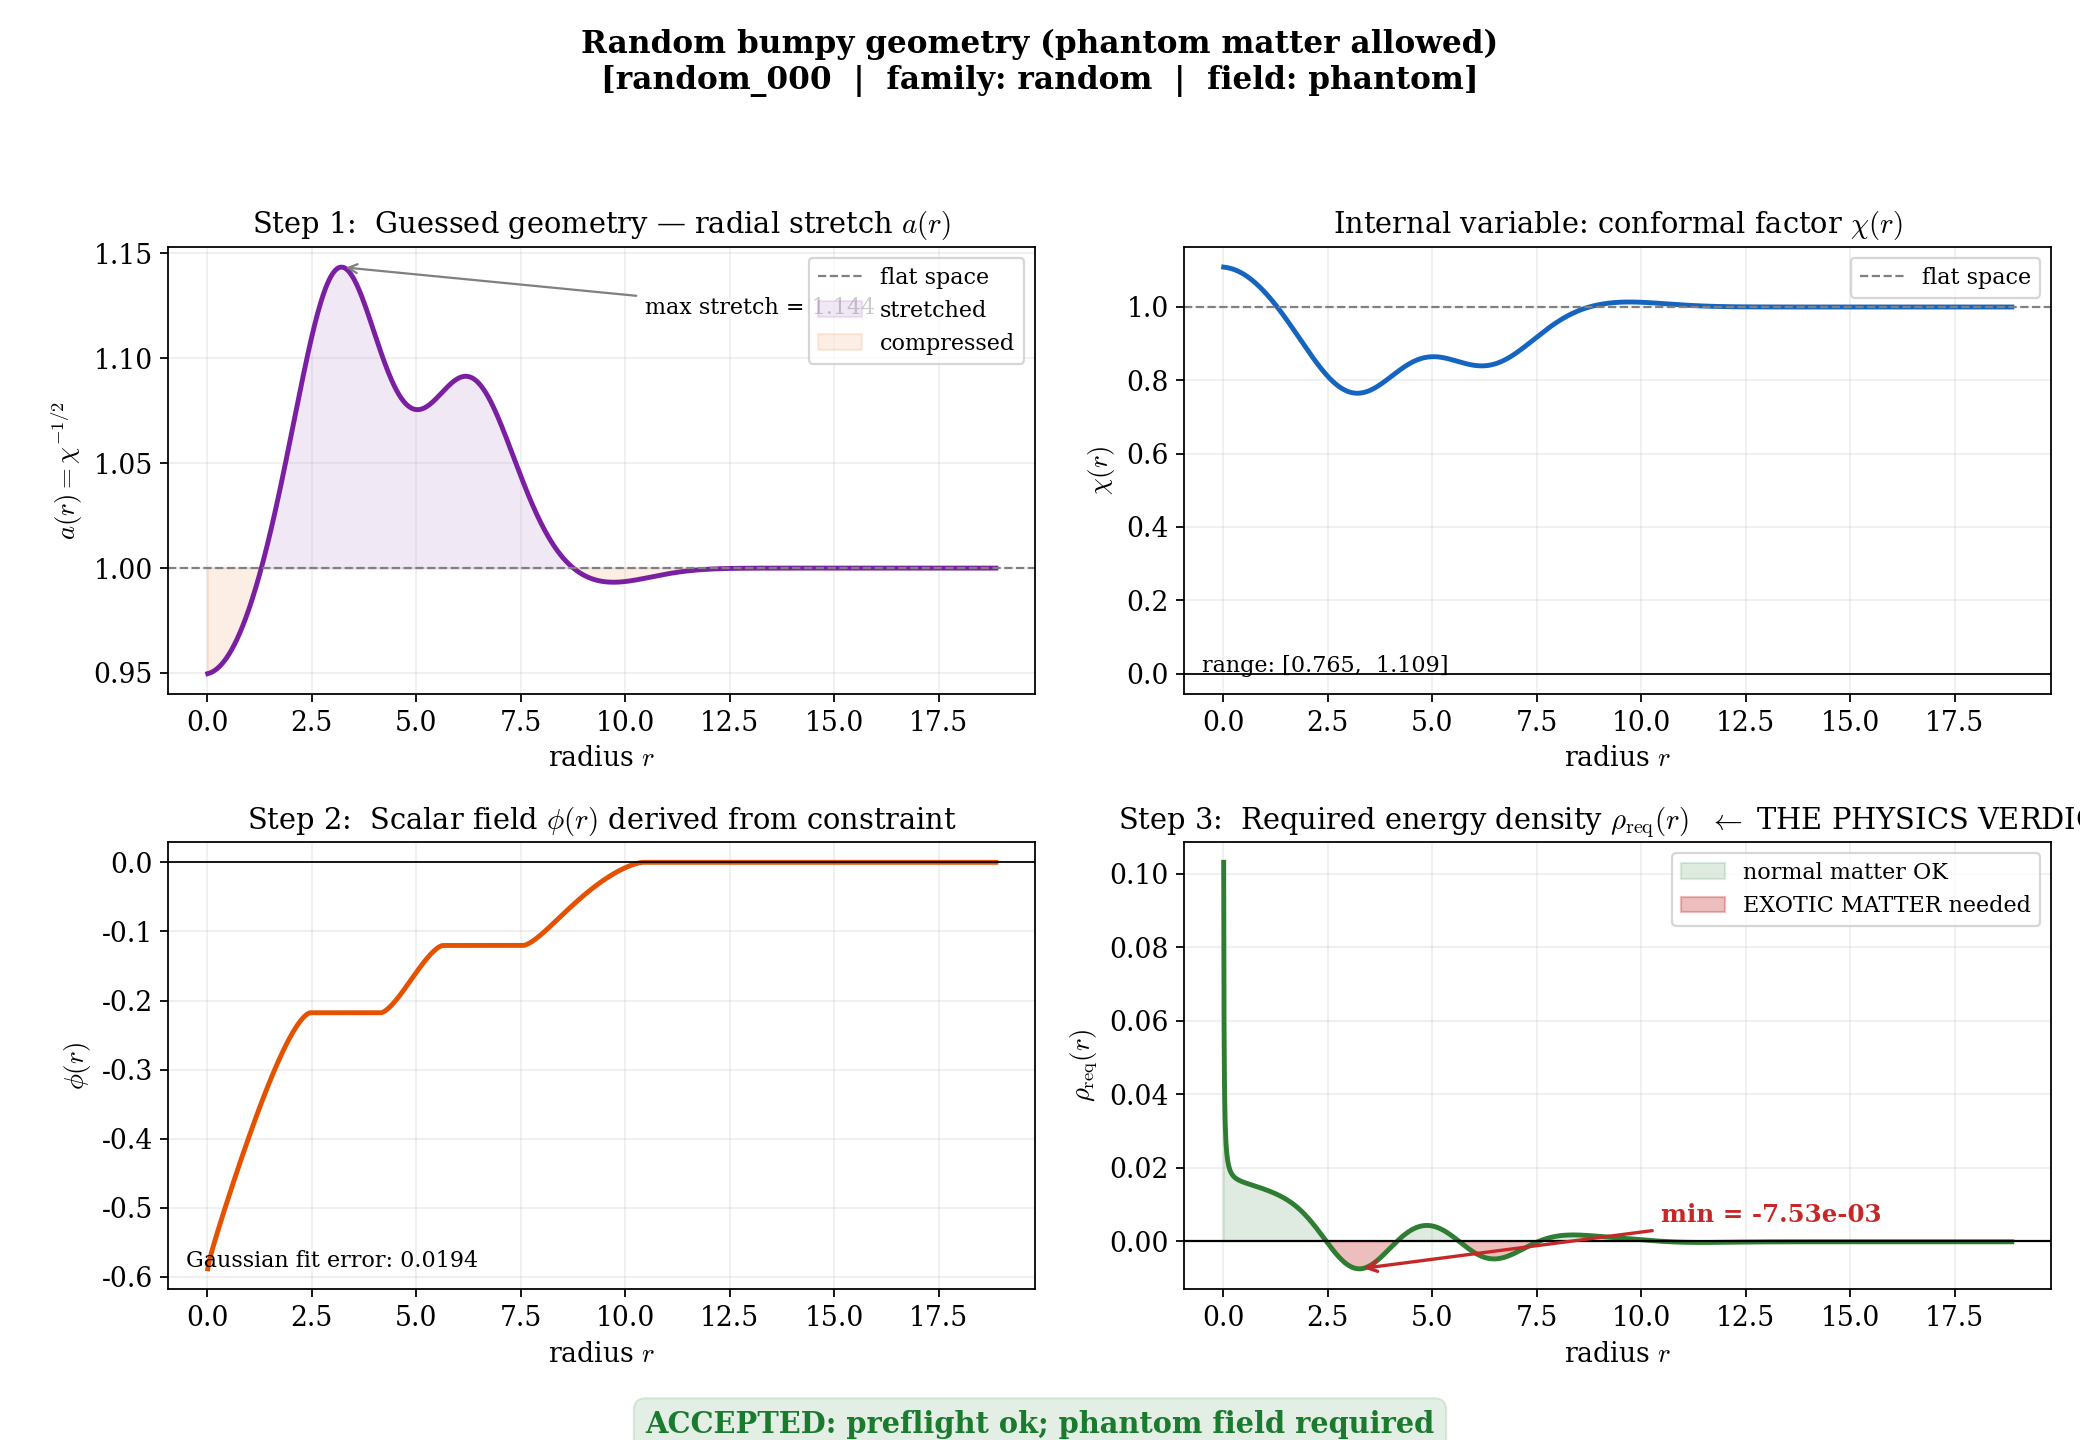
\includegraphics[width=\linewidth,height=0.32\textheight,keepaspectratio]{figures/random_000.png}
    \end{minipage}\hfill
    \begin{minipage}{0.48\textwidth}
        \centering
        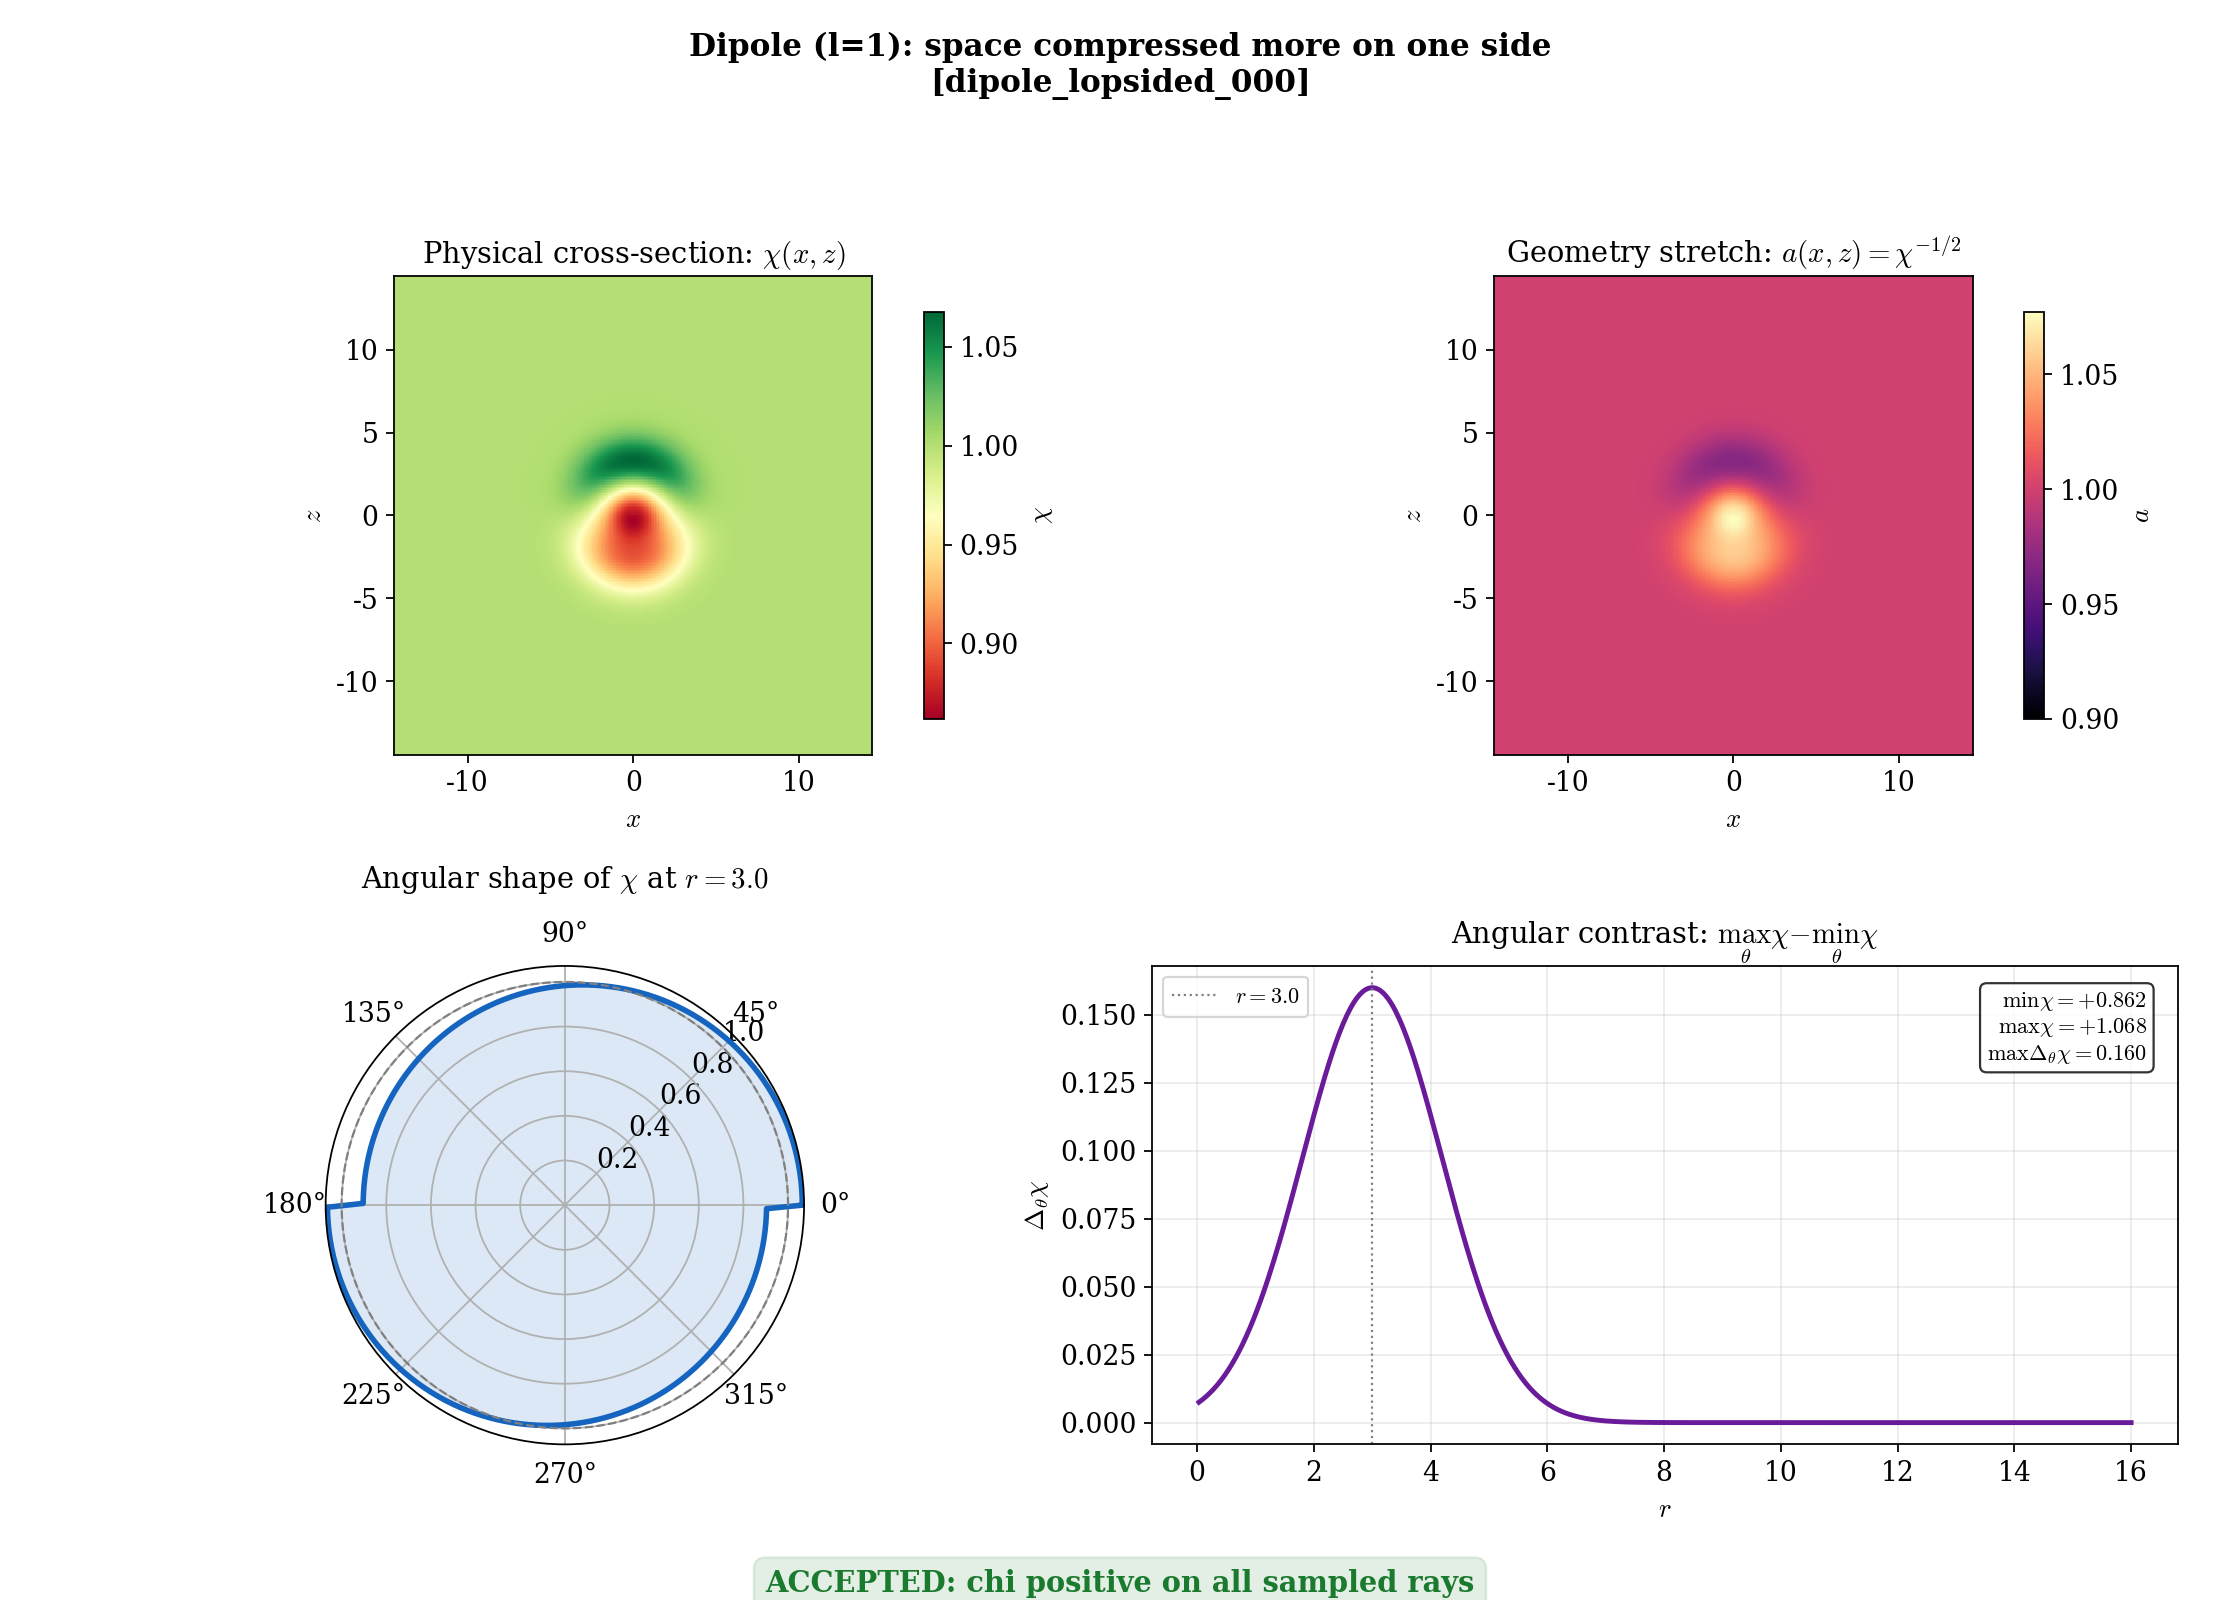
\includegraphics[width=\linewidth,height=0.32\textheight,keepaspectratio]{figures/dipole_lopsided_000.png}
    \end{minipage}
    \caption[Metric-guesser validation examples]{\textbf{Metric-guesser validation examples.} Left: accepted phantom random candidate, showing guessed stretch $a(r)=\chi^{-1/2}$, stored $\chi(r)$, derived scalar $\phi(r)$, and required energy density $\rho_{\rm req}(r)$; it is numerically constructible but accepted only in the phantom/exotic-matter class because $\rho_{\rm req}<0$ in places. Right: accepted non-spherical dipole candidate; the $\ell=1$ mode makes the geometry lopsided while $\chi$ stays positive throughout the ray check.}
    \label{fig:random000}
    \label{fig:nonspherical_dipole}
\end{figure*}

\subsection{GPU/C++ RadialRecipe smoke validation}
\label{sec:gpu_radial_smoke}

The Python wrapper and \path|Examples/RadialRecipe/| executable now run end-to-end on H100 GPUs: generate \texttt{params.txt}, check parameters, evolve, and parse diagnostics.

\subsubsection{Radial smoke results at t=2}

Table~\ref{tab:gpu_radial_smoke} summarizes the first GPU handoff campaign; labels indicate short-run survival only.

\begin{table*}[t]
\caption{Short GPU smoke results for spherically symmetric RadialRecipe candidates ($t=2$, $N_{\rm full}=64$, \texttt{max\_level=0}).  $s_{\rm stability}$ and $S$ are from the eight-component scorer (May 2026 rescoring).  ``Short-run survivor'' means controlled diagnostics over this window, not long-time stability.}
\label{tab:gpu_radial_smoke}
\small
\begin{ruledtabular}
\begin{tabular}{lccccccc}
ID & Python $\|H\|_{L^2}$ & C++ max $\|H\|_{L^2}$ & $\alpha_{\min}$ & $\chi_{\min}$ & $s_{\rm stability}$ & $S$ & Outcome \\
\hline
\texttt{ellis\_bronnikov} & 2.24 & 0.010 & 0.66 & 0.83 & 0.30 & 4.33 & Short-run survivor \\
\texttt{bubble\_wall\_016} & 0.027 & 0.004 & 0.96 & 1.00 & 0.68 & 6.35 & Short-run survivor \\
\texttt{random\_000} & 0.224 & 0.042 & 0.54 & 0.77 & 0.46 & 3.92 & Short-run borderline \\
\end{tabular}
\end{ruledtabular}
\end{table*}

The 3D diagnostics stay controlled even when the coarse 1D pre-flight residual is conservative.  Extended $t=5$ tests promote Ellis--Bronnikov and \texttt{bubble\_wall\_016} to the resolution ladder.

\subsubsection{Resolution note (Ellis--Bronnikov)}

Increasing $N_{\rm full}$ from 64 to 128 sharpens the Ellis--Bronnikov throat while keeping constraints controlled.

\subsubsection{AMR closed-loop test}

The first full-domain AMR CMA-ES run found only low-stability survivors (Table~\ref{tab:amr_optimize}), confirming the stop-time exploit that the growth metric targets.

\begin{table*}[t]
\caption{Top AMR CMA-ES candidates (\texttt{optimize\_20260528T055206Z}, $t=2$, stability-aware scoring).}
\label{tab:amr_optimize}
\small
\begin{ruledtabular}
\begin{tabular}{lccccc}
Eval & $S$ & $s_{\rm stability}$ & $\alpha_{\min}$ & $\chi_{\min}$ & $|K|_{\max}$ \\
\hline
\texttt{eval\_000013} & 4.12 & 0.085 & 0.29 & 0.47 & 1.02 \\
\texttt{eval\_000006} & 4.05 & 0.056 & 0.24 & 0.41 & 2.33 \\
\texttt{eval\_000009} & 4.00 & 0.054 & 0.19 & 0.35 & 2.39 \\
\texttt{eval\_000002} & 3.87 & 0.049 & 0.07 & 0.29 & 1.84 \\
\texttt{eval\_000015} & 2.21 & 0.035 & 0.00 & 0.06 & 1.73 \\
\end{tabular}
\end{ruledtabular}
\end{table*}

\subsection{Non-spherical 3D GPU batch}
\label{sec:gpu_nonspherical}

All seven ray-sane non-spherical candidates survive short GPU evolution with controlled constraints (Table~\ref{tab:gpu_nonspherical}).

\begin{table*}[t]
\caption{Non-spherical GPU smoke results ($t=2$, $N_{\rm full}=64$, stability-aware scoring).}
\label{tab:gpu_nonspherical}
\small
\begin{ruledtabular}
\begin{tabular}{lccccc}
Candidate & max $\|H\|_{L^2}$ & $\alpha_{\min}$ & $\chi_{\min}$ & $s_{\rm stability}$ & $S$ \\
\hline
\texttt{dipole\_lopsided\_000} & 0.0118 & 0.90 & 0.88 & 0.44 & 4.93 \\
\texttt{quadrupole\_bubble\_001} & 0.0125 & 0.92 & 0.87 & 0.50 & 4.98 \\
\texttt{mixed\_modes\_002} & 0.0118 & 0.91 & 0.87 & 0.44 & 4.89 \\
\texttt{random\_angular\_004} & 0.0064 & 0.92 & 0.87 & 0.50 & 5.31 \\
\texttt{random\_angular\_005} & 0.0122 & 0.91 & 0.87 & 0.49 & 4.98 \\
\texttt{random\_angular\_006} & 0.0132 & 0.91 & 0.87 & 0.49 & 4.97 \\
\texttt{random\_angular\_007} & 0.0135 & 0.92 & 0.87 & 0.51 & 4.98 \\
\end{tabular}
\end{ruledtabular}
\end{table*}

Their stability scores exceed the AMR-optimized radial survivors but remain below true-equilibrium values.

\subsection{Gauge-sector angular search and streaming HQ validation (implemented)}
\label{sec:gauge_angular_search}

Because angular $\chi$ cannot be made constraint-consistent by a 1D solve, we next opened the gauge sector: $\alpha$ and $\beta^i$ carry Legendre modes with $\ell\in\{1,2\}$ and searchable radial centers/widths, giving a 21-parameter gauge-angular space.

\paragraph{Search outcome.}  An 8-GPU campaign found evolved superluminal channels at $\int\!\rho_{-}\,dV\approx0.13$--$0.17$, a factor $2$--$5$ below spherical persistent-FTL candidates.  The top candidate, \texttt{eval\_000188}, was promoted.

\paragraph{Streaming high-quality validation.}  \texttt{eval\_000188} was re-evolved to $t=16$ at $N_{\rm full}=192$, \texttt{max\_level=2}, with on-the-fly plotfile consumption and deletion, keeping the full validation near $1.2$\,GB.

The validated geometry is a standing Alcubierre-like $\chi$ dipole, not a translating bubble: the evolved channel persists weakly by $t=16$, constraints decrease, and exotic matter remains small and axial, but a near-trapped flag appears in the compressed lobe.

\begin{table}[tbp]
\caption{High-quality streaming validation of the gauge-angular winner \texttt{eval\_000188} ($N_{\rm full}=192$, \texttt{max\_level=2}, $t=16$, H100).  Initial vs.\ evolved operational FTL, exotic matter, and constraint health.}
\label{tab:hq188}
\small
\begin{ruledtabular}
\begin{tabular}{p{0.53\columnwidth}c}
Quantity & Value \\
\hline
$\max c$ (initial slice)            & $2.67$ \\
$\max c$ (evolved, $t=16$)          & $1.32$ \\
$F_{\rm op}^{0}$ / $F_{\rm op}^{\rm ev}$ & $0.35$ / $5.6\times10^{-3}$ \\
superluminal path fraction (evolved) & $0.51$ \\
$\int\rho_{-}\,dV$ (exotic matter)  & $0.134$ \\
ANEC line integral (axis)           & $-6.6\times10^{-3}$ \\
$\|H\|_{L^2}$ (max / final)         & $1.1\times10^{-3}$ / $4.2\times10^{-4}$ \\
$\|M\|_{L^2}$ (final)               & $3.6\times10^{-5}$ \\
$\min\theta_+$ (near-trapped flag)  & $-0.11$ \\
$S$ (gated total)                   & $16.75$ \\
\end{tabular}
\end{ruledtabular}
\end{table}

\begin{figure}[tbp]
    \centering
    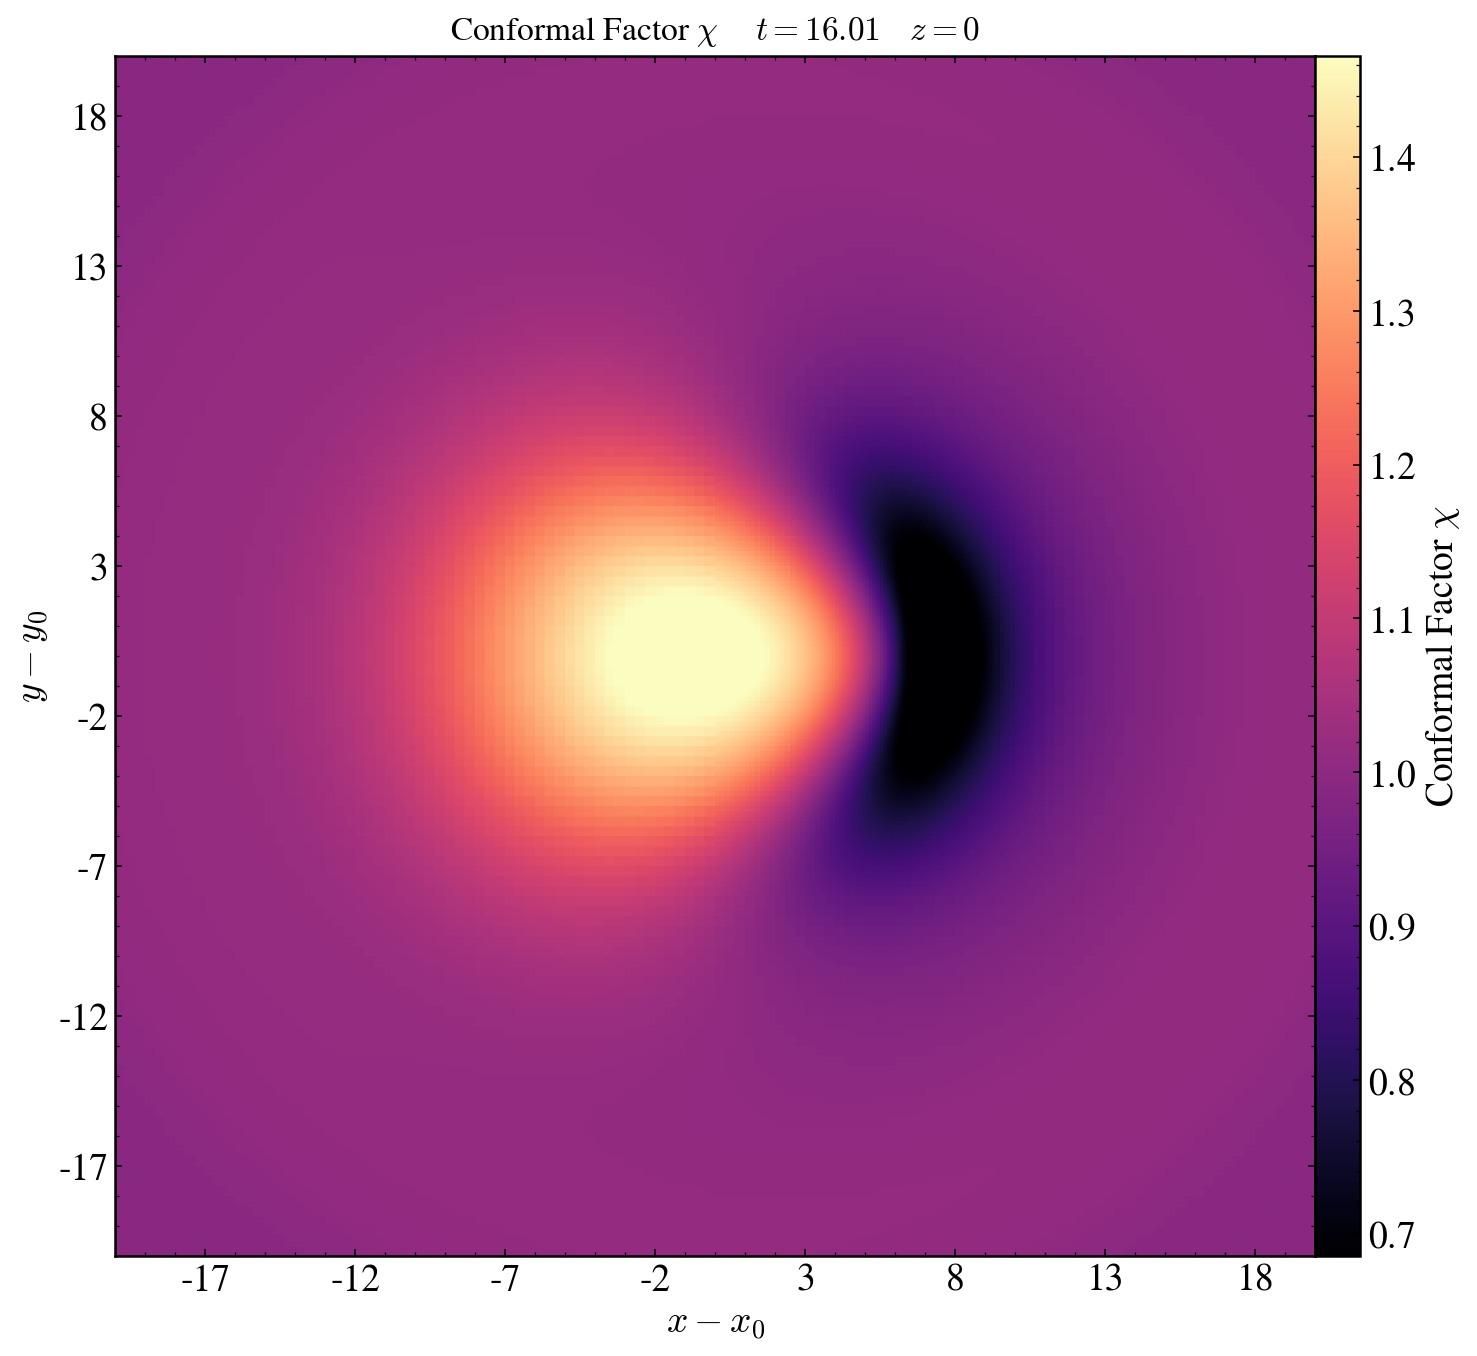
\includegraphics[width=0.85\columnwidth]{articlepictures/hq188_chi_t16.png}
    \caption{\textbf{Persistent directional channel of the gauge-angular winner \texttt{eval\_000188}} (conformal factor $\chi$, $z=0$ slice, $t=16$, $N_{\rm full}=192$).  A standing front--back dipole compresses space on the $+x$ side ($\chi\approx0.7$, dark) and expands it behind ($\chi\approx1.45$, bright)---an Alcubierre-like contract-ahead/expand-behind polarity realized through the shift sector at low exotic-matter cost.  The structure does not translate; it stands and slowly decays.  Frames were extracted on the fly during evolution while plotfiles were deleted (keep-last-2).}
    \label{fig:hq188}
\end{figure}

\paragraph{Why not a wormhole or portal.}  The current parameterization cannot change topology, and its non-spherical freedom lives in the gauge sector, where shift structure naturally favors warp-like channels.  Wormholes and portals require topology search plus a 3D constraint solver.

\section{Forward Path: From Stability Gap to Analytic Discovery}
\label{sec:forward_path}

The main remaining challenge is the dynamical stability gap: optimizers can still favor geometries that merely outlive a short stop time.  The production path is:

\subsection{Phase 1: Closing the stability gap (immediate software priority)}

Use $s_{\rm growth}$ to reject positive growth, calibrate it against $t=5$--$10$ ladders, keep the FTL scaffolding/gated objective active, and sweep basis size/width before promotion.

\subsection{Directional non-spherical search: next degrees of freedom}
\label{sec:directional_next}

Gauge-angular search produced a low-exotic directional channel.  Next degrees of freedom are:

\begin{enumerate}
    \item searchable radial placement of angular modes;
    \item full-$z$ domains without reflective parity;
    \item persistence/co-motion rewards;
    \item soft barriers on near-trapped surfaces;
    \item higher angular order and a dedicated translation shift.
\end{enumerate}

\paragraph{The geometric sector.}  The largest improvement is a 3D elliptic constraint solver, allowing directional structure in $\chi$ or $\tilde A_{ij}$ without reintroducing off-axis constraint error.

\paragraph{Topology search.}  Wormholes and portals require a discrete controller that selects mouths, throats, modes, and boundary connectivity before the continuous optimizer refines each topology.

\subsection{Phase 2: Multi-observer energy conditions}
\label{sec:warp_factory_methods}

The $t=0$ ANEC and tidal proxies are blind to pure-shift warps, so \texttt{warpfactory.py} evaluates energy conditions from the evolved 4-metric via $T_{\mu\nu}=G_{\mu\nu}/8\pi$, e.g.
\begin{equation}
    \Xi_W(\mathbf{x}) = \min_{V}\,T_{\mu\nu}\,V^{\mu}V^{\nu},\qquad g_{\mu\nu}V^\mu V^\nu=-1,
\end{equation}
This recovers Alcubierre NEC/WEC violations missed by $\chi$-sourced proxies.

The evaluator also uses a Hawking--Ellis/Type-I hybrid margin following \textsc{warpax}~\cite{le2026warpax}, with fourth-order finite differences~\cite{lousto2006fourth}; its margin feeds \texttt{score.py} as $s_{\rm exotic}^{\rm eff}$.

\subsection{Phase 3: GPU-cluster production search}

With surrogate screening, MAP-Elites, and Pareto extraction in place, production runs are a 1000-candidate constraint atlas plus a 50-generation CMA-ES campaign:
\begin{verbatim}
python -m grteclyn_wrapper \
    --example RadialRecipe \
    --constrained --preflight optimize \
    --max-generations 50 --seed 42
\end{verbatim}

\subsection{Phase 4: Analytical back-derivation}

A numerical optimum is only a coefficient list.  The final handoff reconstructs $\chi_{\rm num}$, fits a closed form by symbolic regression, solves the Hamiltonian constraint for $\phi(r)$, and reloads the analytic profile for verification.  This can be automated as a multi-agent loop inspired by \textsc{PhysAgent}~\cite{han2025physagent}.

\section{Extensions: Implemented Metrics, Search, and Robustness}
\label{sec:proposed}

The extensions below target three limits: short-run gaming, coordinate-dependent energy/FTL verdicts, and expensive GPU evaluations.

\subsection{New physical metrics}

\paragraph{Constraint growth rate.}  Fit late-time diagnostics to $q(t)\sim q_0e^{\lambda t}$ and penalize the worst growth:
\begin{equation}
    \begin{aligned}
    s_{\rm growth}
    &= r\!\left(\max(0,\lambda_{\rm eff});\,\sigma_\lambda\right),\\
    \lambda_{\rm eff}
    &= \max\!\bigl(\lambda_{\|H\|},\,\lambda_{|K|_{\max}},\,\lambda_{1/\chi_{\min}}\bigr),
    \end{aligned}
    \label{eq:s_growth}
\end{equation}
with $\sigma_\lambda=0.5$.

\paragraph{ANEC line proxy.}  Integrate required energy along the travel axis:
\begin{equation}
    \begin{aligned}
    \mathcal{A}_{\rm line}
    &= \int_{-L}^{L}\rho_{\rm req}(x)\,dx,\\
    s_{\rm anec}
    &= r\!\left(\max(0,-\mathcal{A}_{\rm line});\,\sigma_{\mathcal A}\right),
    \end{aligned}
    \label{eq:anec_line}
\end{equation}
with $\rho_{\rm req}=(R+\tfrac{2}{3}K^2)/16\pi$ and $\sigma_{\mathcal A}=0.1$.  The full target is
\begin{equation}
    \mathcal{A} = \int_\gamma T_{\mu\nu}\,k^\mu k^\nu\,d\lambda,
    \label{eq:anec}
\end{equation}
which requires the evolved probe and a local tetrad.

\paragraph{Tidal proxy.}  Use $T_{\rm tidal}=\max_x|R(x)|+\max_x|\partial_x^2\alpha(x)|$ and a $t=0$ trapped-surface flag until full 4-curvature diagnostics are available.

\paragraph{Operational probe FTL.}  Compare first arrival on the candidate and an identical flat control:
\begin{equation}
    F_{\rm op} = \frac{t_B^{\rm flat} - t_B^{\rm curved}}{t_B^{\rm flat}},
    \label{eq:f_op}
\end{equation}
accepted only with no trapped-surface crossing and bounded constraints.

Table~\ref{tab:phys_t0} gives reference $t=0$ proxy values.

\begin{table*}[t]
\caption{Implemented $t=0$ gauge-robust proxies on reference seeds ($L=8$, 1024 points).  $\mathcal{A}_{\rm line}$ is the axis energy-density line integral (Eq.~\ref{eq:anec_line}); $\mathcal{K}^{1/2}_{\rm proxy}\equiv\max|R|$ is the spatial-curvature scale; ``trap'' is the $t=0$ trapped-surface flag.}
\label{tab:phys_t0}
\small
\begin{ruledtabular}
\begin{tabular}{lccccc}
Seed & $\mathcal{A}_{\rm line}$ & $s_{\rm anec}$ & $\max|R|$ & $s_{\rm tidal}$ & trap \\
\hline
Flat Minkowski & $0$ & 1.000 & $0$ & 1.000 & no \\
Alcubierre $v{=}0.5$ & $0$ & 1.000 & $0$ & 1.000 & no \\
Ellis--Bronnikov & $-6.62$ & 0.015 & $2.0{\times}10^{4}$ & 0.000 & yes \\
Schwarzschild & $-2.38$ & 0.040 & $6.0{\times}10^{3}$ & 0.000 & yes \\
\end{tabular}
\end{ruledtabular}
\end{table*}

Table~\ref{tab:gpu_growth} shows that every short-run survivor still has positive $\lambda_{\rm eff}$, exposing the stability gap from a single smoke run.

\begin{table*}[t]
\caption{GPU growth-rate and new-component values ($t=2$, $N_{\rm full}=64$, \texttt{max\_level=0}).  $\lambda_{\rm eff}$ from Eq.~\eqref{eq:s_growth}; $S$ is the total under the extended 15-component scorer (adds $s_{\rm growth},s_{\rm anec},s_{\rm tidal}$ to Table~\ref{tab:score_weights}).}
\label{tab:gpu_growth}
\small
\begin{ruledtabular}
\begin{tabular}{lccccc}
Candidate & $\lambda_{\rm eff}$ & $s_{\rm growth}$ & $s_{\rm anec}$ & $s_{\rm tidal}$ & $S$ \\
\hline
\texttt{alcubierre\_warp} & 0.99 & 0.335 & 1.000 & 1.000 & 13.25 \\
\texttt{ellis\_bronnikov} & 1.02 & 0.329 & 0.015 & 0.000 & 12.18 \\
\texttt{bubble\_wall\_016} & 0.41 & 0.550 & 0.987 & 0.524 & 10.76 \\
\texttt{random\_000} & 0.29 & 0.633 & 0.682 & 0.161 & 7.57 \\
\end{tabular}
\end{ruledtabular}
\end{table*}

\subsection{Optimizing the search}

\paragraph{Surrogate-assisted screening.}  \texttt{surrogate.py} uses an RBF kernel-ridge model to pre-screen CMA-ES proposals; one 8-GPU run skipped 27\% of GPU evaluations while retaining the best score.

\paragraph{Quality-Diversity.}  \texttt{qd\_search.py} maintains MAP-Elites over FTL benefit and exoticity, producing a diverse failure atlas rather than a single optimum.

\begin{table}[tbp]
\caption{MAP-Elites archive from one $40$-evaluation, 8-GPU campaign ($6{\times}6$ grid, coverage $0.19$).  Each row is the elite of a distinct behavior cell.}
\label{tab:qd_atlas}
\small
\begin{ruledtabular}
\begin{tabular}{cccc}
Cell & FTL benefit & Exoticity & Elite $S$ \\
\hline
$(1,0)$ & 0.319 & 0.000 & 12.47 \\
$(3,1)$ & 0.618 & 0.248 & 12.13 \\
$(2,0)$ & 0.384 & 0.000 & 11.68 \\
$(3,0)$ & 0.595 & 0.040 & 11.62 \\
$(0,0)$ & 0.000 & 0.000 & 10.98 \\
$(1,1)$ & 0.332 & 0.228 & 10.21 \\
$(0,1)$ & 0.160 & 0.231 & 9.91 \\
\end{tabular}
\end{ruledtabular}
\end{table}

\paragraph{Pareto front.}  \texttt{pareto.py} reports non-dominated candidates over $(F_{\rm FTL},s_{\rm anec},s_{\rm growth},s_{\rm tidal})$, exposing trade-offs hidden by scalar weights.

\paragraph{Constraint-solved initial data.}  Making elliptic Path~B the default is the largest single improvement: every proposal would start constraint-satisfying, reducing junk radiation and making growth rates cleaner.

\section{Conclusion}

This work turns exotic-metric study into a closed-loop GPU search over dynamical initial data.  The current pipeline proposes constrained recipes, evolves them in \texttt{GRTeclyn}, scores stability/FTL/energy diagnostics, and validates promising candidates on longer runs.  The first campaigns expose the central stability gap but also show that FTL scaffolding, non-triviality gating, growth metrics, evolved energy-condition checks, surrogate screening, MAP-Elites, and Pareto extraction can steer the search away from trivial flat space.  The next step is a 3D elliptic constraint solver and topology-aware search, enabling genuinely geometric warp, portal, and wormhole candidates to be tested with observer-robust physical diagnostics.

\begin{thebibliography}{9}

\bibitem{alexander2026albert}
S.~Alexander, B.~Bradley, L.~Gouskos, and C.~Niu,
\newblock ``Autonomous Discovery of Particle Physics Theories from Experimental Data,''
\newblock arXiv:2603.28935 [hep-ph] (2026).

\bibitem{qiu2026collideragent}
S.~Qiu, Z.~Cai, J.~Wei, Z.~Li, Y.~Yin, Q.-H.~Cao, C.~Liu, M.-x.~Luo, X.-B.~Yuan, and H.~X.~Zhu,
\newblock ``An End-to-end Architecture for Collider Physics and Beyond,''
\newblock arXiv:2603.14553 [hep-ph] (2026).

\bibitem{halverson2019branes}
J.~Halverson, B.~Nelson, and F.~Ruehle,
\newblock ``Branes with Brains: Exploring String Vacua with Deep Reinforcement Learning,''
\newblock JHEP \textbf{06}, 003 (2019), arXiv:1903.11616 [hep-th].

\bibitem{han2025physagent}
X.-Q.~Han, Z.-F.~Gao, P.-J.~Guo, and Z.-Y.~Lu,
\newblock ``PhysAgent: A Multi-Agent Approach to Automated Discovery of Physical Laws,''
\newblock arXiv preprint (2025).

\bibitem{helmerich2024warpfactory}
C.~Helmerich, J.~Fuchs, A.~Bobrick, L.~Sellers, B.~Melcher, and G.~Martire,
\newblock ``Analyzing Warp Drive Spacetimes with Warp Factory,''
\newblock Class.\ Quantum Grav.\ (2024), arXiv:2404.03095 [gr-qc].

\bibitem{le2026warpax}
A.~T.~Le,
\newblock ``Observer-robust energy condition verification for warp drive spacetimes,''
\newblock arXiv:2602.18023 [gr-qc] (2026).

\bibitem{lousto2006fourth}
C.~O.~Lousto,
\newblock ``A time-domain fourth-order-convergent numerical algorithm to integrate black hole perturbations in the extreme-mass-ratio limit,''
\newblock Class.\ Quantum Grav.\ \textbf{22}, S543 (2005), arXiv:gr-qc/0503001.

\bibitem{li2023pinn}
Z.-H.~Li, C.-Q.~Li, and L.-G.~Pang,
\newblock ``Solving Einstein equations using deep learning,''
\newblock arXiv:2309.07397 [gr-qc] (2023).

\end{thebibliography}

\end{document}